\chapter{Project Breakdown Structure}
For better understanding of the projects composition, the following explains its inner Structure and the different components its made up of.

\begin{figure}[h]
	\centering
	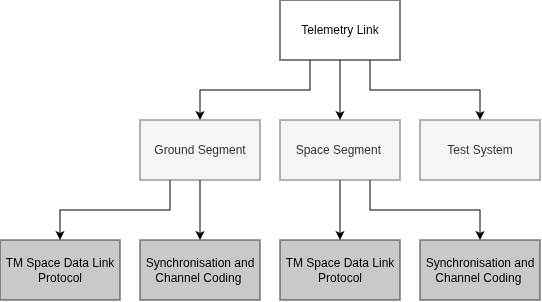
\includegraphics[width=0.7\linewidth]{img/ProjectStructure.png}
	\caption{Project Structure}
	\label{fig:project_structure}
\end{figure}

The entire project can firstly be divided into 3 main subsystems shown by figure \ref{fig:project_structure}. The TM Segment on Ground and its counterpart referred to as Space Segment, as well the necessary Test System for Hardware in the Loop testing planned towards the end of project. Both Ground and Space Segment are further divided into the implementation of the TM Space Data Link Protocol described in CCSDS 132.0-B-3 and the Synchronization and Channel Coding of CCSDS 131.0-B-5.